%!TEX root = ../../main.tex
\section{Specifikation og Analyse}
\label{sec:specandanal}
Ud fra opgaveformuleringen er der blevet skrevet en kravspecifikation. Kravspecifikationen specificerer hvilke krav, der er til \gls{system}et. Såsom hvordan \gls{system}et skal se ud til hvordan skal håndtere et handlingsforløb. Det er i \gls{usecase}s, at et handlingsforløb mellem aktør og \gls{system}et er beskrevet. Ved analyse er det også \gls{usecase}s, der kigges på.
\newline\newline
Først og fremmest er der blevet lavet en domænemodel. Domænemodellen kan findes i afsnittet DomainView i systemarkitekturen. Domænemodellen er en metode, hvor man danner et klassediagram ud fra de fully dressed \gls{usecase}s. Klassediagrammet viser ikke videre, hvordan klasserne skal implementeres, men hjælper til at give et overblik over hvilke ansvar, som skal håndteres i \gls{system}et. Klassediagrammet skal fungere, som inspiration til det videre design. 
\newline\newline
I Figur~\ref{fig:domainmodel} kan et udsnit af domænemodellen for \gls{system}et ses. Udtræk af domænemodellen kan ses i den nuværende system implementering og andre ting er blevet smidt væk. F.eks. er \texttt{CashRegister} klassen i figuren blevet splittet op i to klasser: \texttt{Sales} og \texttt{Orders}.

\begin{figure}[H]
	\centering
	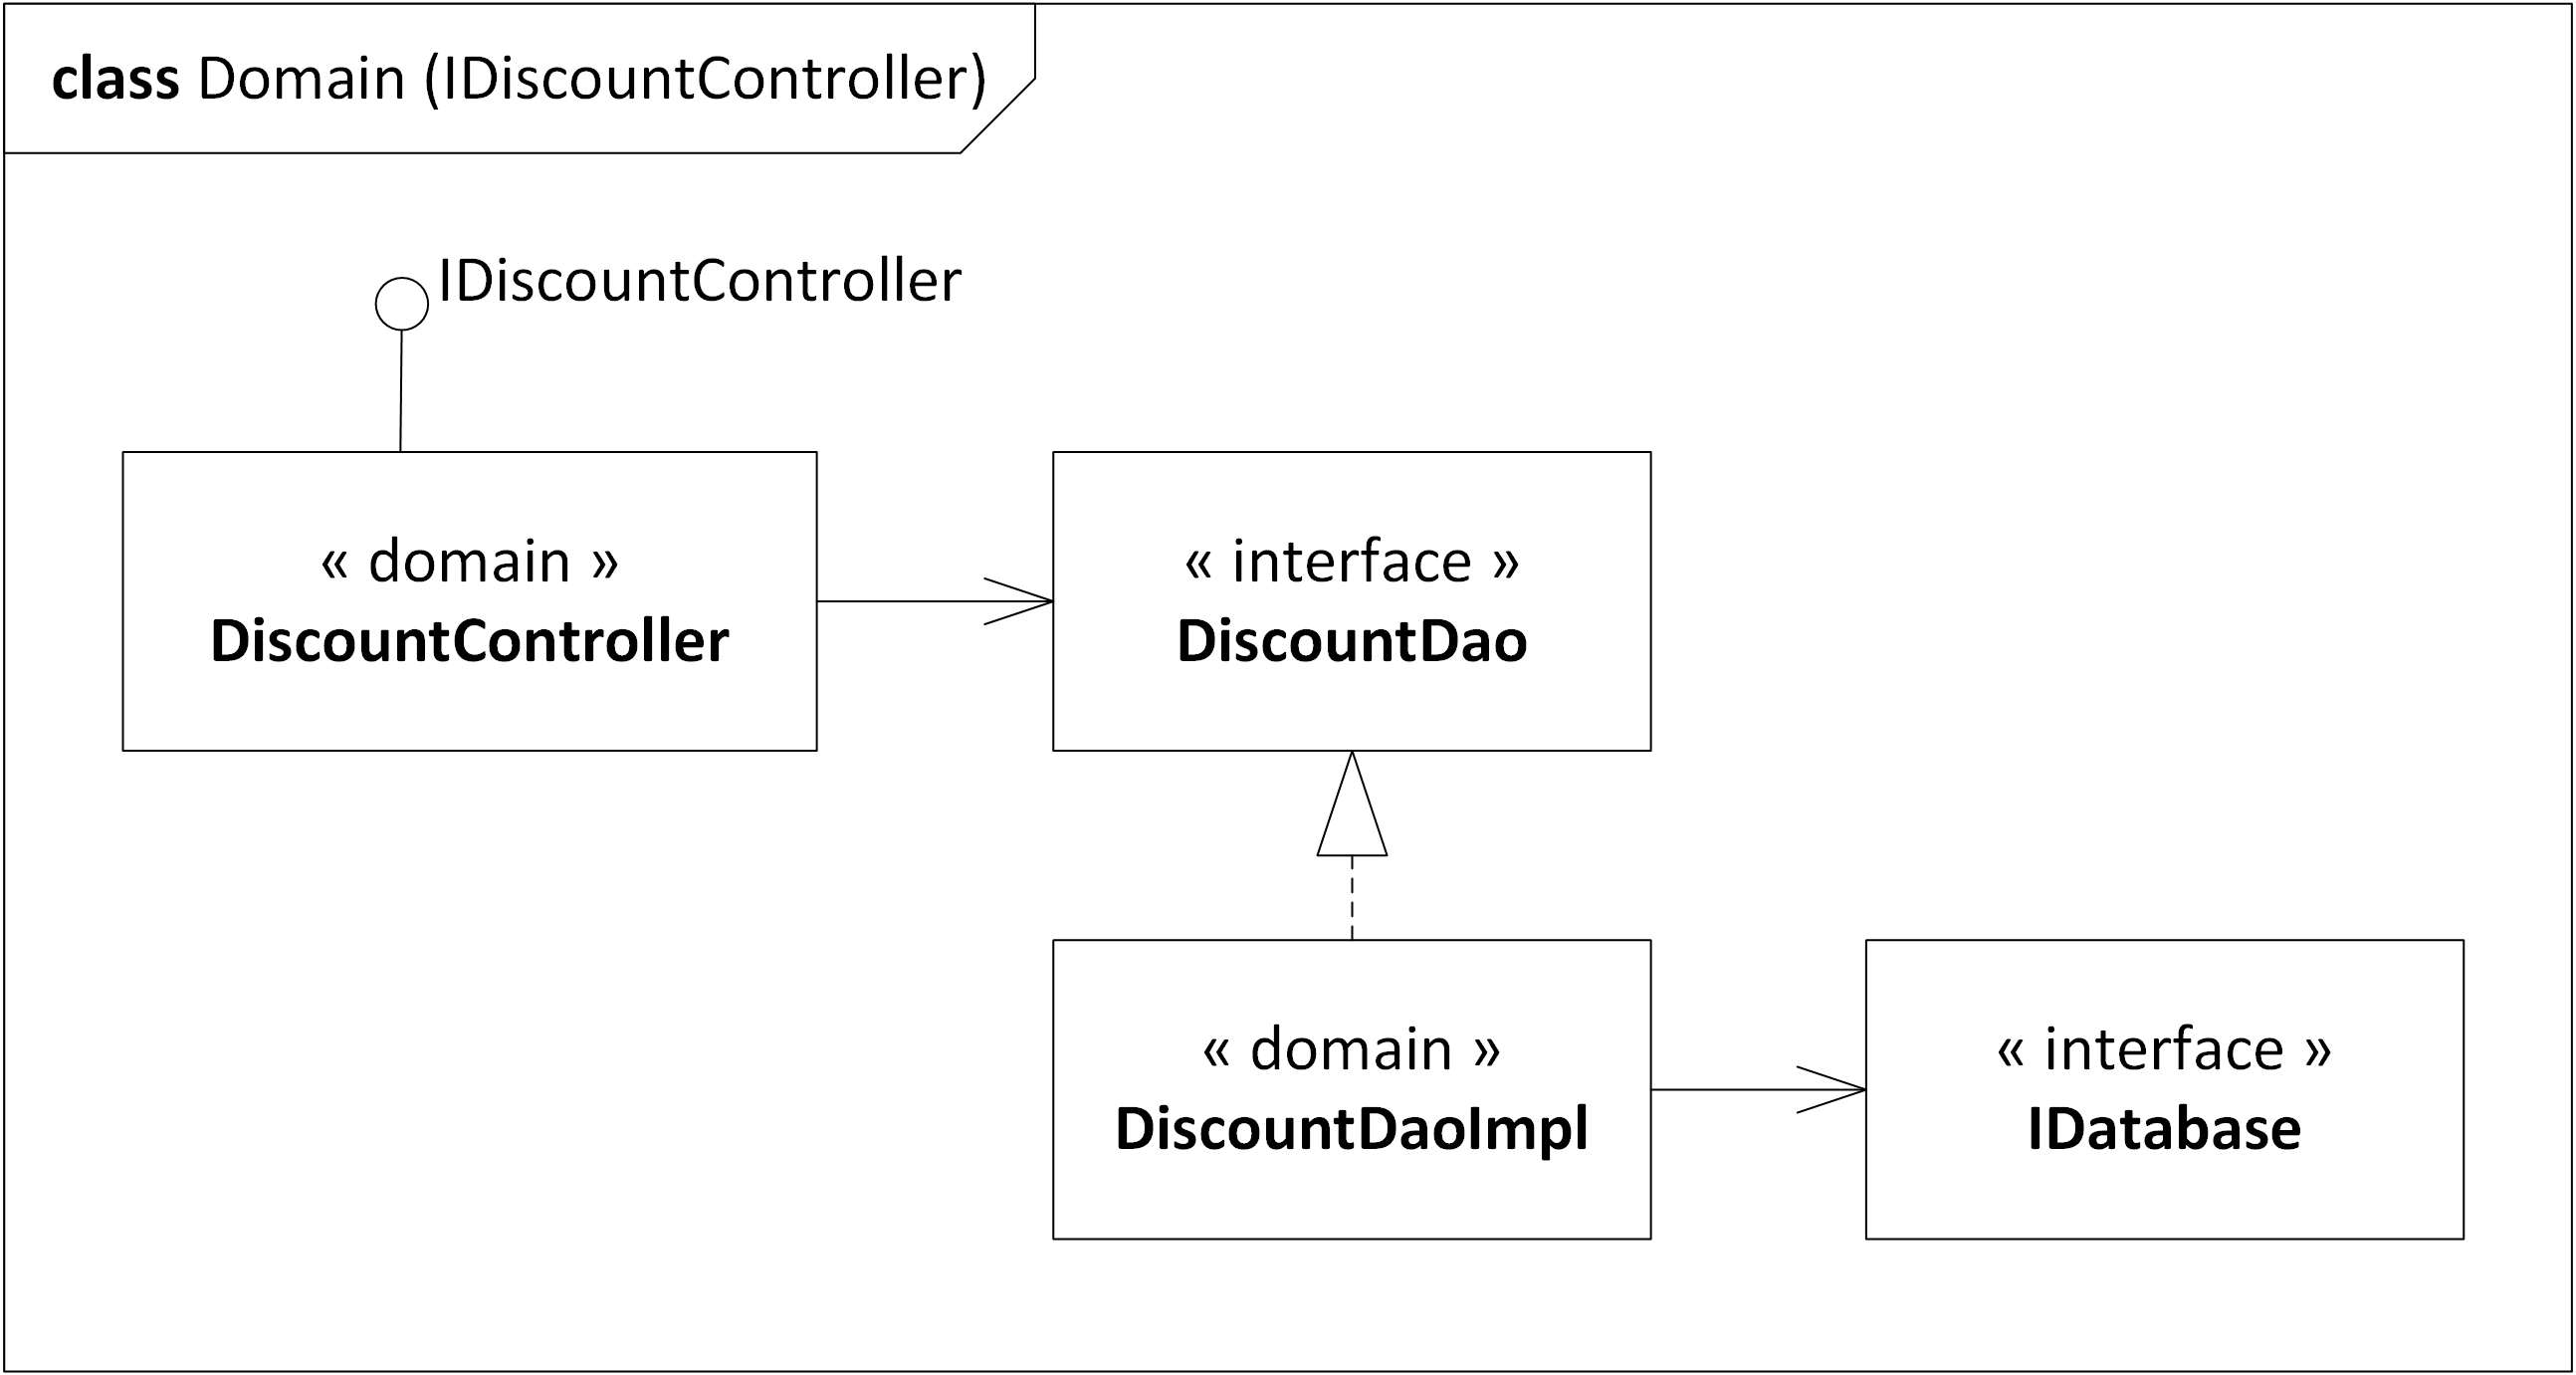
\includegraphics[width=0.95\textwidth]{N+1/DomainView/CashRegister/Diagrammer/DOMAIN.png}
	\caption{Domænemodel for \Gls{system}et}
	\label{fig:domainmodel}
\end{figure}

En anden del af analysen kan findes i afsnittet UseCaseView i systemarkitekturen. Her er de fully dressed \gls{usecase}s sat op i sekvensdiagrammer. Formålet er at vise, hvordan \gls{system}et svarer på input. Dette er især en hjælp til \gls{GUI}, som er brugerens indgang til systemet. I Figur~\ref{fig:usecaseviewseq} kan \gls{usecase} 1 ses. Her vises handlingsforløbet med respons og hvordan det kommer til udtryk i \gls{GUI}.

\begin{figure}[H]
	\centering
	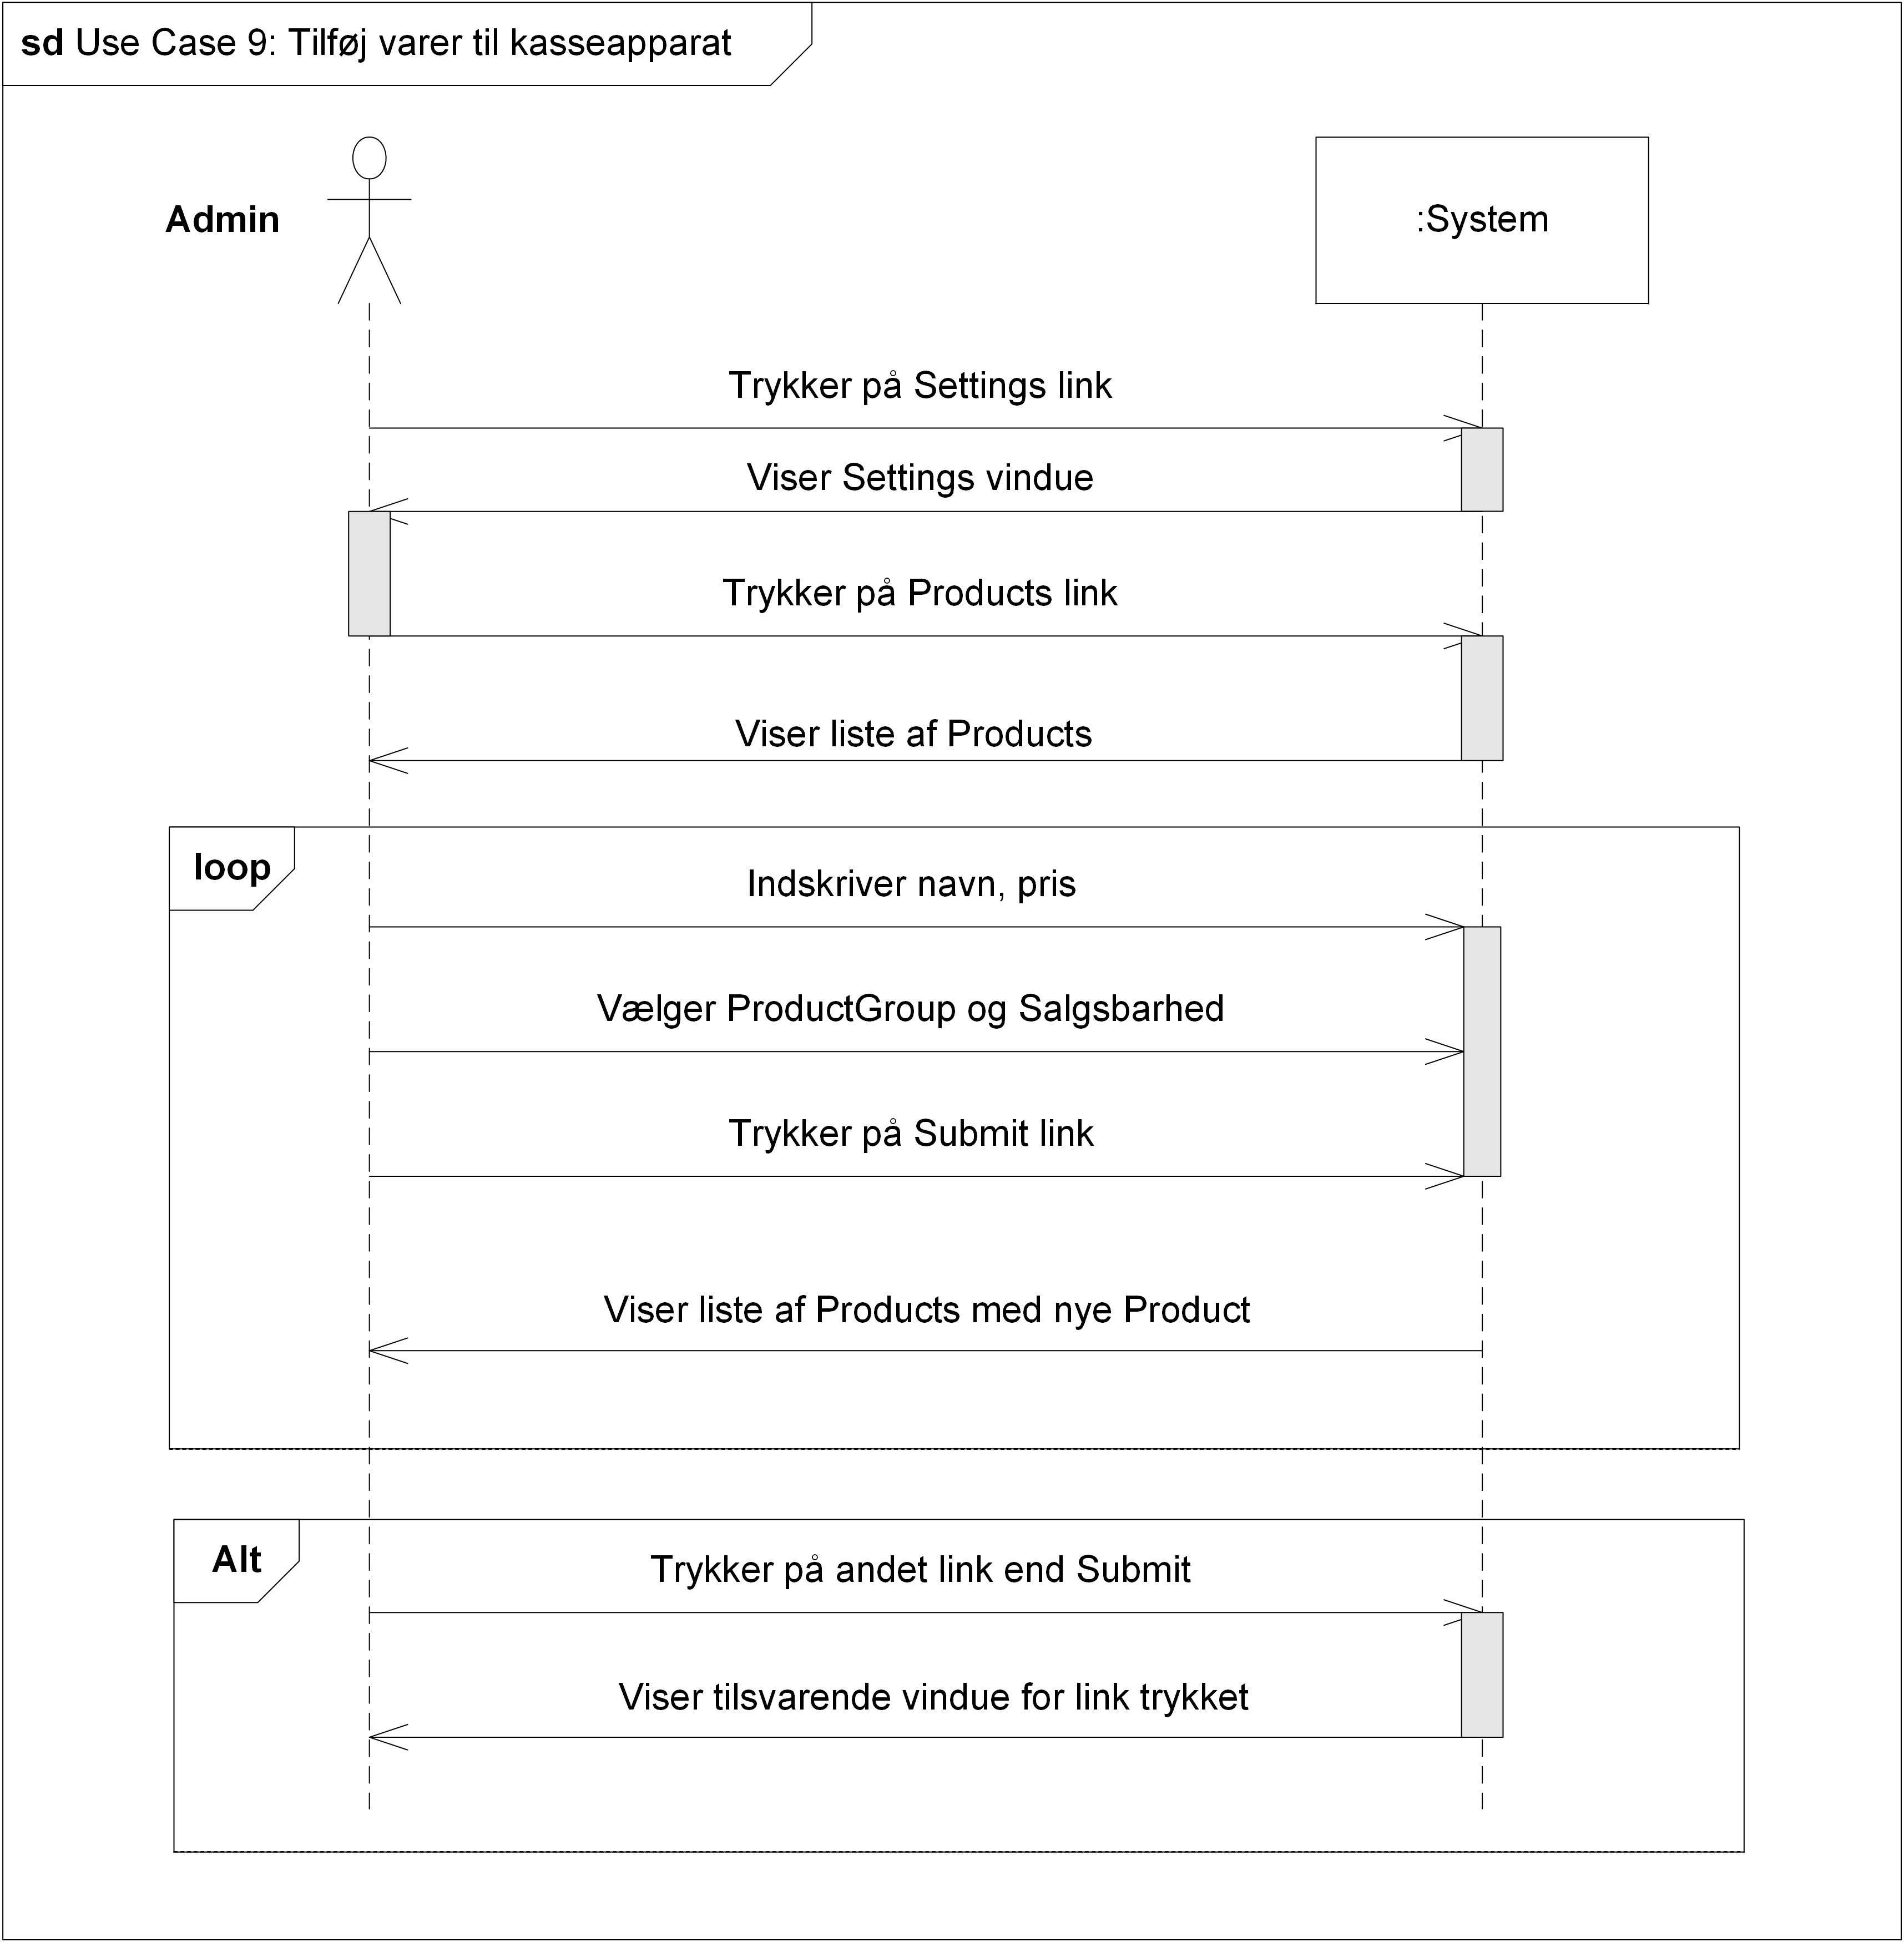
\includegraphics[width=0.6\textwidth]{N+1/UseCaseView/UseCase1/Diagrammer/SEQ.png}
	\caption{Et sekvensdiagram over \gls{usecase} 1}
	\label{fig:usecaseviewseq}
\end{figure}